The goal of this work is to reduce the effort required to produce high-quality gaze animation modeling the gaze behavior as an automatically inferrable, easily editable sequence of gaze instances. %In this section, we present two evaluations we conducted to gauge our success: the first evaluation measured the authoring effort required to author and edit gaze using our approach in comparison with a traditional tool
We conducted a two-part evaluation of our approach. The first experiment assesses the amount of effort required to author gaze animations to confirm that our approach does save animator time and effort. The second experiment assesses the quality of the resulting animations, to ensure that sufficient quality is maintained.

\subsection{Authoring Effort}
\label{sec:GazeAuthoringEffortEvaluation}

We evaluated authoring effort in two ways. First, we investigated the effort required to add eye animation to a captured body motion without modifying the motion itself---something our tool can do automatically. We had two experienced animators add eye movements to seven scenes, originally captured for the gaze inference evaluation (Section ~\ref{sec:GazeAuthoringEffortEvaluation}), with cumulative length of 2:36 minutes. Both animators used Autodesk MotionBuilder, where they set up a simple eye animation rig, which they keyed to create the desired eye movements. We measured authoring effort using two metrics: (1) time taken and (2) number of keys set. We found that the animators required on average 25 minutes and 86 keys per minute of animation. By contrast, our system can synthesize an equivalent amount of eye animation automatically, requiring on average 90 seconds of computation per minute of animation.

Second, we assessed the effort required to edit gaze animation in a scene which already contained eye movements. An experienced animator was instructed to make the following edits: (1) introduce gaze aversion in a two-character interaction scene (HandShake), (2) remove gaze toward an object in an environment interaction scene (StealGem), (3) introduce gaze toward a new character in a multi-character interaction scene (DrinkSoda), and (4) introduce gaze toward the camera in an environment interaction scene (MakeSandwich). The edits in all the scenes involved changing not just eye movements, but also head and (in some cases) torso posture. To accomplish the edits, the animator used layering and keyframing features in MotionBuilder. Meanwhile, a novice animator authored the same edits using our gaze editing tool. As before, we measured time taken and number of operations required. For MotionBuilder, the latter is equivalent to the number of keys set, while for our tool, it refers to the editing operations discussed in Section~\ref{sec:GazeEditing}. The results, reported in Table~\ref{tab:GazeEditingEffortResults}, suggest equivalent edits may be achievable using our approach in 1/5 of the time and with 1/3 the number of operations required by traditional motion editing.
%
\begin{table}
\centering
\def\arraystretch{1.5}
\begin{tabular}{|l||l|l|l|l|}
\hline
\textbf{Scene} & \multicolumn{2}{l|}{\textbf{Traditional}} & \multicolumn{2}{l|}{\textbf{Our Approach}} \\
\cline{2-5}
& Time & \# keys & Time & \# ops  \\
\hline
HandShake & 10:40 & 19 & 3:11 & 8 \\
StealGem & 1:29 & 9 & 1:30 & 4 \\
DrinkSoda & 9:05 & 43 & 3:51 & 9 \\
MakeSandwich & 10:43 & 33 & 4:05 & 13 \\
\hline
\end{tabular}
\caption{Gaze editing effort: traditional vs. our approach.}
\label{tab:GazeEditingEffortResults}
\end{table}
%
\subsection{Animation Quality}
\label{sec:GazeAnimationQualityEvaluation}

To evaluate the effect of our gaze authoring approach on perceived quality of produced animation, we conducted a human subjects experiment. We compared our approach to other methods of gaze animation production: no eye animation, eye movements recorded using an eye tracker, and hand-authored gaze. We showed participants pairs of videos of a motion-captured character performing various actions and asked them to choose the one they thought had superior animation. The videos in each pair were identical in every way except the gaze animation method. Different methods corresponded to the following study conditions: (1) \emph{no gaze}, (2) \emph{recorded gaze} (using an eye tracker), (3) \emph{hand-authored gaze}, and (4) \emph{synthesized gaze} (our approach.)

\noindent\textbf{Hypotheses} -- We hypothesized the following: (1) \emph{Synthesized gaze} would be preferred over \emph{no gaze}. (2) \emph{Synthesized gaze} would be preferred over \emph{recorded gaze}. (3) \emph{Synthesized gaze} would be seen as equivalent to \emph{hand-authored gaze}. Hypothesis 2 is motivated by the consideration that raw eye-tracking data is noisy, non-trivial to map to an animated character, and often incorrect with respect to scene requirements. Hypothesis 3 reflects the expectation that our approach can synthesize gaze animation at a level of quality approaching hand-authoring.

\noindent\textbf{Design} -- The experiment involved three separate studies, each of which tested one of the hypotheses. Each study consisted of five task trials and followed a within-participants design, wherein the participants were asked to choose between videos in \emph{synthesized gaze} and one of the other conditions. Video pairs were presented to the participants in a randomized order.

\noindent\textbf{Stimuli} -- Experiment stimuli were $5 \times 4$ video clips (five scenes, each in four conditions) of a character animated using motion capture, 9 to 14 seconds in length. We created the \emph{no gaze} condition videos by extracting segments original scenes created for the gaze inference evaluation (Section~\ref{sec:GazeInferenceEvaluation}.) The scenes were: ChatWithFriend, MakeSandwich, StackBoxes, StealGem, WalkCones. The \emph{hand-authored gaze} condition was created by extracting those same segments from the scenes created for the authoring effort evaluation (Section~\ref{sec:GazeAuthoringEffortEvaluation}), while the \emph{synthesized gaze} condition was the result of applying our gaze inference to the segments. To create the \emph{recorded gaze} condition, we generated eye animations directly from eye tracking data.

\noindent\textbf{Measures} -- Our experiment had the following subjective measures: (1) perceived \emph{animator competence}, (2) \emph{realism}, and (3) \emph{communicative clarity}. The measures were implemented as binary-choice questions the participant answered on each task trial: (1) ``On which video did the animator do a better job?'' (2) ``In which video were the character\'s movements more realistic?'' (3) ``In which video did the character communicate more clearly what they were doing?''

\noindent\textbf{Participants} -- We conducted the experiment online using Amazon Mechanical Turk crowdsourcing service. We recruited 24 participants for each study---a total of 72 participants. The participants were paid at the rate of \$6/hour.
% TODO: Did you collect any demographics? I think people will at least expect gender breakdown.

\noindent\textbf{Results} -- Upon collecting our data, we conducted separate analyses for each study of the experiment. We aggregated all participants' binary answers across all the scenes and obtained, for each condition, the count of how many times it was chosen over its counterpart in each measure. Then we compared the counts using chi-square tests of goodness-of-fit. The results, shown in~\ref{fig:StudyResults}, were as follows.

\begin{figure}[t]
\centering
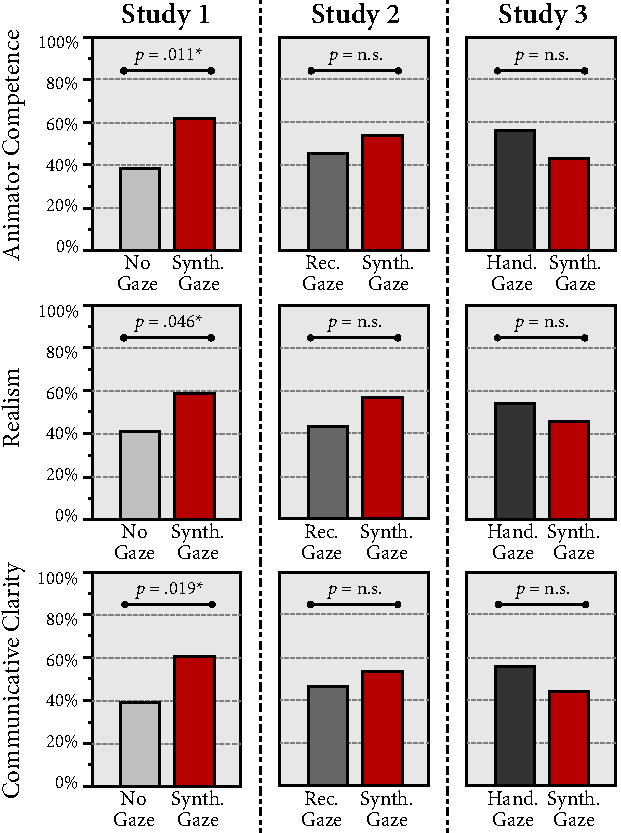
\includegraphics[width=0.48\textwidth]{Figures/StudyResults.pdf}
\caption{Results of the study comparing gaze animation produced using our approach (\emph{Synthesized Gaze}) to (1) no gaze animation, (2) gaze recorded using an eye tracker, and (3) hand-authored gaze. y-axis shows the percentage of trials in which one condition was chosen over the other.}
\label{fig:StudyResults}
\end{figure}

Our analysis of data from study one found a significant preference for \emph{synthesized gaze} over \emph{no gaze} on all measures: $\chi^2(1, 120) = 6.41, p = .011*$ (animator competence), $\chi^2(1, 120) = 3.99, p = .046*$ (realism), and $\chi^2(1, 120) = 5.54, p = .019*$ (communicative clarity.) These results constitute support for Hypothesis 1.

Data from the second study showed that \emph{synthesized gaze} was not significantly preferred over \emph{recorded gaze} in any of the measures: $\chi^2(1, 120) = 0.83, p = .362$ (animator competence), $\chi^2(1, 120) = 2.12, p = .145$ (realism), and $\chi^2(1, 120) = 0.53, p = .466$ (communicative clarity.) Therefore, we did not find support for Hypothesis 2.

In study three, chi-square test results were the following: $\chi^2(1, 120) = 2.12, p = .145$ (animator competence), $\chi^2(1, 120) = 0.83, p = .362$ (realism), and $\chi^2(1, 120) = 1.63, p = .202$ (communicative clarity.) While there was no significant difference in preference between \emph{synthesized gaze} and \emph{hand-authored gaze} on any of the measures, $p$-values also did not reach the suggested equivalence margin of $p \geq .50$~\cite{walker2011equivalence}, indicating lack of support for Hypothesis 3.

In a post-hoc exploratory analysis, we investigated the potential reasons for the lack of support for Hypothesis 2, as the findings contrasted our own observations. This analysis focused on how recorded and synthesized gaze differed across different scenarios in order to determine whether or not our approach had a differential effect on different scenes. We found that scene type had a significant effect on participants' choice of \emph{recorded gaze} in all measures (e.g., $\chi^2(4, 55) = 25.04, p < .0001^*$ for the ``animator competence'' measure). Further inspection showed that scenes with a close-up of the character benefited the most from our synthesized gaze approach, likely due to greater saliency of gaze cues. The differences between approaches were indiscernible in scenes where the character's eyes were small on the screen and other motion components dominated. An illustrative example is the ChatWithFriend scene, which was always chosen in \emph{synthesized gaze} condition over \emph{recorded gaze} in animator competence and realism measures, and 23 times out of 24 in communicative clarity.
%ChatWithFriend scene was always chosen in \emph{synthesized gaze} condition over \emph{recorded gaze} in animator competence and realism measures, and 23 times out of 24 in communicative clarity. We believe that is because ChatWithFriend scene showed a close-up of the character and placed emphasis on the gaze animation, which would have brought attention to high-frequency artifacts in recorded gaze and reduced the confounding effects of other animation components.
%In other scenes, where the eyes are small and other animation components dominate, it is unsurprising that we do not see a strong preference

Study results suggest that gaze animation is important for the perception of animation quality, and adding gaze animation using our approach leads to improvement in perceived animation quality. Benefits of gaze authoring may be more pronounced in scenes where gaze behavior is perceptually dominant. Finally, while we found no conclusive evidence that gaze authored by a trained expert was superior to the output of our method, we also did not find that they were equivalent in quality.
\begin{comment}
\subsection{Effectiveness of Editing}

HandShake
    1. How much was the green character focusing on the blue character?
        OG: $(M = 90.83\%, SD = 10.84)$
        NEG: $(M = 33.33\%, SD = 37.50)$
        $t(13) = -5.10, p = .0002*$
    2. How much was the green character focusing on the floor?
        OG: $(M = 21.67\%, SD = 31.57)$
        NEG: $(M = 82.50\%, SD = 21.79)$
        $t(20) = -5.49, p < .0001*$

MakeSandwich
    1. How much was the blue character focusing on the tabletop?
        OG: $(M = 62.50\%, SD = 27.01)$
        NEG: $(M = 54.17\%, SD = 22.75)$
        $t(21) = -0.81, p = .4227$
    2. How much was the blue character focusing on the camera?
        OG: $(M = 26.67\%, SD = 23.48)$
        NEG: $(M = 45.00\%, SD = 22.76)$
        $t(22) = 1.94, p = .0065$

PassSoda:
    1. How much was the blue character focusing on the green character?
        OG: $(M = 93.33\%, SD = 7.79)$
        NEG: $(M = 34.17\%, SD = 25.53)$
        $t(13) = -8.27, p < .0001*$
    2. How much was the blue character focusing on the pink character?
        OG: $(M = 5.00\%, SD = 7.98)$
        NEG: $(M = 70.83\%, SD = 22.75)$
        $t(14) = 9.46, p < .0001*$
        
StealGem
    1. How much was the blue character focusing on the red gem?
        OG: $(M = 79.17\%, SD = 25.75)$
        NEG: $(M = 50.00\%, SD = 41.78)$
        $t(18) = -2.06, p = .054$
    2. How much was the blue character focusing on the yellow gem?
        OG: $(M = 10.83\%, SD = 22.75)$
        NEG: $(M = 10.83\%, SD = 22.75)$
        $t(22) = 0, p = 1$

TODO: add figure StudyResults2
\end{comment}